% This file is generated by the MATLAB m-file laprint.m. It can be included
% into LaTeX documents using the packages graphicx, color and psfrag.
% It is accompanied by a postscript file. A sample LaTeX file is:
%    \documentclass{article}\usepackage{graphicx,color,psfrag}
%    \begin{document}% This file is generated by the MATLAB m-file laprint.m. It can be included
% into LaTeX documents using the packages graphicx, color and psfrag.
% It is accompanied by a postscript file. A sample LaTeX file is:
%    \documentclass{article}\usepackage{graphicx,color,psfrag}
%    \begin{document}% This file is generated by the MATLAB m-file laprint.m. It can be included
% into LaTeX documents using the packages graphicx, color and psfrag.
% It is accompanied by a postscript file. A sample LaTeX file is:
%    \documentclass{article}\usepackage{graphicx,color,psfrag}
%    \begin{document}% This file is generated by the MATLAB m-file laprint.m. It can be included
% into LaTeX documents using the packages graphicx, color and psfrag.
% It is accompanied by a postscript file. A sample LaTeX file is:
%    \documentclass{article}\usepackage{graphicx,color,psfrag}
%    \begin{document}\input{onedimlp}\end{document}
% See http://www.mathworks.de/matlabcentral/fileexchange/loadFile.do?objectId=4638
% for recent versions of laprint.m.
%
% created by:           LaPrint version 3.16 (13.9.2004)
% created on:           19-Oct-2009 10:48:43
% eps bounding box:     20 cm x 12.8261 cm
% comment:              
%
\begin{psfrags}%
\psfragscanon%
%
% text strings:
\psfrag{s02}[b][b]{\color[rgb]{0,0,0}\setlength{\tabcolsep}{0pt}\begin{tabular}{c}$J(z)$\end{tabular}}%
\psfrag{s05}[l][l]{\color[rgb]{0,0,0}\setlength{\tabcolsep}{0pt}\begin{tabular}{l}$\mathcal{R_1}$ \end{tabular}}%
\psfrag{s06}[l][l]{\color[rgb]{0,0,0}\setlength{\tabcolsep}{0pt}\begin{tabular}{l}$\mathcal{R}_3$ \end{tabular}}%
\psfrag{s07}[l][l]{\color[rgb]{0,0,0}\setlength{\tabcolsep}{0pt}\begin{tabular}{l}$\mathcal{R}_4$ \end{tabular}}%
\psfrag{s08}[l][l]{\color[rgb]{0,0,0}\setlength{\tabcolsep}{0pt}\begin{tabular}{l}$\mathcal{R}_2$ \end{tabular}}%
\psfrag{s09}[l][l]{\color[rgb]{0,0,0}\setlength{\tabcolsep}{0pt}\begin{tabular}{l}$z$ \end{tabular}}%
\psfrag{s10}[l][l]{\color[rgb]{0,0,0}\setlength{\tabcolsep}{0pt}\begin{tabular}{l}$c_1'z+d_1$ \end{tabular}}%
\psfrag{s15}[l][l]{\color[rgb]{0,0,0}\setlength{\tabcolsep}{0pt}\begin{tabular}{l}$c_2'z+d_2$ \end{tabular}}%
\psfrag{s16}[l][l]{\color[rgb]{0,0,0}\setlength{\tabcolsep}{0pt}\begin{tabular}{l}$c_3'z+d_3$ \end{tabular}}%
\psfrag{s17}[l][l]{\color[rgb]{0,0,0}\setlength{\tabcolsep}{0pt}\begin{tabular}{l}$c_4'z+d_14$ \end{tabular}}%
%
% xticklabels:
\psfrag{x01}[t][t]{0}%
\psfrag{x02}[t][t]{0.1}%
\psfrag{x03}[t][t]{0.2}%
\psfrag{x04}[t][t]{0.3}%
\psfrag{x05}[t][t]{0.4}%
\psfrag{x06}[t][t]{0.5}%
\psfrag{x07}[t][t]{0.6}%
\psfrag{x08}[t][t]{0.7}%
\psfrag{x09}[t][t]{0.8}%
\psfrag{x10}[t][t]{0.9}%
\psfrag{x11}[t][t]{1}%
\psfrag{x12}[t][t]{0}%
\psfrag{x13}[t][t]{0.1}%
\psfrag{x14}[t][t]{0.2}%
\psfrag{x15}[t][t]{0.3}%
\psfrag{x16}[t][t]{0.4}%
\psfrag{x17}[t][t]{0.5}%
\psfrag{x18}[t][t]{0.6}%
\psfrag{x19}[t][t]{0.7}%
\psfrag{x20}[t][t]{0.8}%
\psfrag{x21}[t][t]{0.9}%
\psfrag{x22}[t][t]{1}%
\psfrag{x23}[t][t]{0}%
\psfrag{x24}[t][t]{1}%
\psfrag{x25}[t][t]{2}%
\psfrag{x26}[t][t]{3}%
\psfrag{x27}[t][t]{4}%
\psfrag{x28}[t][t]{5}%
\psfrag{x29}[t][t]{6}%
\psfrag{x30}[t][t]{7}%
%
% yticklabels:
\psfrag{v01}[r][r]{0}%
\psfrag{v02}[r][r]{0.1}%
\psfrag{v03}[r][r]{0.2}%
\psfrag{v04}[r][r]{0.3}%
\psfrag{v05}[r][r]{0.4}%
\psfrag{v06}[r][r]{0.5}%
\psfrag{v07}[r][r]{0.6}%
\psfrag{v08}[r][r]{0.7}%
\psfrag{v09}[r][r]{0.8}%
\psfrag{v10}[r][r]{0.9}%
\psfrag{v11}[r][r]{1}%
\psfrag{v12}[r][r]{0}%
\psfrag{v13}[r][r]{0.1}%
\psfrag{v14}[r][r]{0.2}%
\psfrag{v15}[r][r]{0.3}%
\psfrag{v16}[r][r]{0.4}%
\psfrag{v17}[r][r]{0.5}%
\psfrag{v18}[r][r]{0.6}%
\psfrag{v19}[r][r]{0.7}%
\psfrag{v20}[r][r]{0.8}%
\psfrag{v21}[r][r]{0.9}%
\psfrag{v22}[r][r]{1}%
\psfrag{v23}[r][r]{-1}%
\psfrag{v24}[r][r]{0}%
\psfrag{v25}[r][r]{1}%
\psfrag{v26}[r][r]{2}%
\psfrag{v27}[r][r]{3}%
\psfrag{v28}[r][r]{4}%
\psfrag{v29}[r][r]{5}%
\psfrag{v30}[r][r]{6}%
%
% Figure:
\resizebox{16cm}{!}{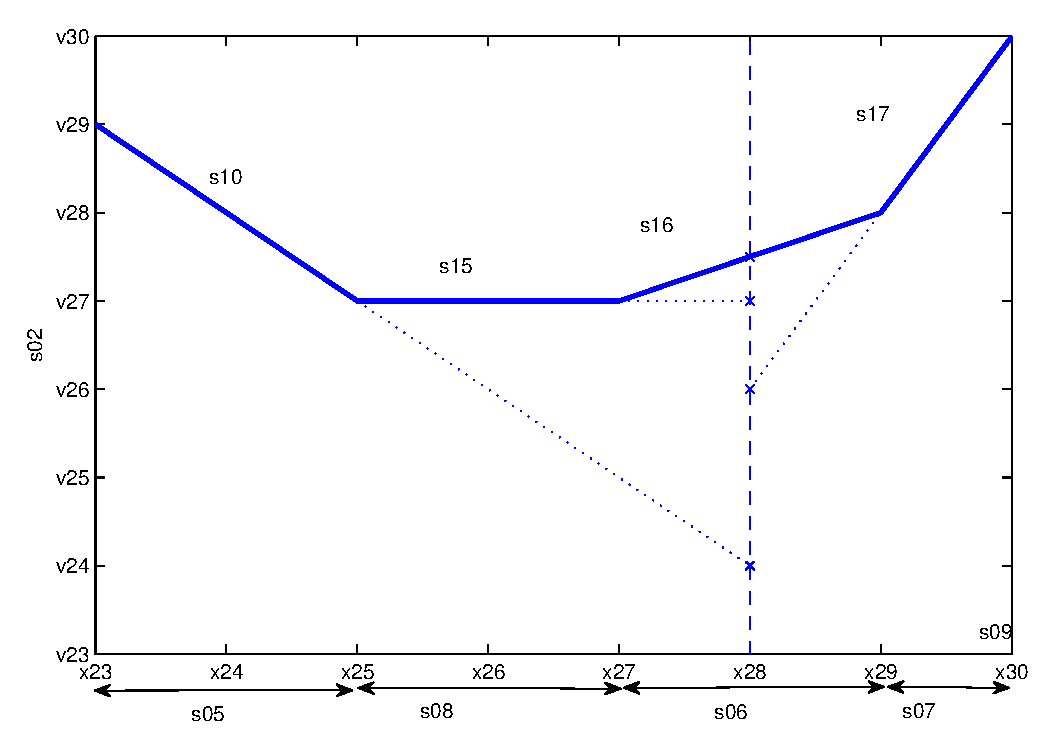
\includegraphics{onedimlp.eps}}%
\end{psfrags}%
%
% End onedimlp.tex
\end{document}
% See http://www.mathworks.de/matlabcentral/fileexchange/loadFile.do?objectId=4638
% for recent versions of laprint.m.
%
% created by:           LaPrint version 3.16 (13.9.2004)
% created on:           19-Oct-2009 10:48:43
% eps bounding box:     20 cm x 12.8261 cm
% comment:              
%
\begin{psfrags}%
\psfragscanon%
%
% text strings:
\psfrag{s02}[b][b]{\color[rgb]{0,0,0}\setlength{\tabcolsep}{0pt}\begin{tabular}{c}$J(z)$\end{tabular}}%
\psfrag{s05}[l][l]{\color[rgb]{0,0,0}\setlength{\tabcolsep}{0pt}\begin{tabular}{l}$\mathcal{R_1}$ \end{tabular}}%
\psfrag{s06}[l][l]{\color[rgb]{0,0,0}\setlength{\tabcolsep}{0pt}\begin{tabular}{l}$\mathcal{R}_3$ \end{tabular}}%
\psfrag{s07}[l][l]{\color[rgb]{0,0,0}\setlength{\tabcolsep}{0pt}\begin{tabular}{l}$\mathcal{R}_4$ \end{tabular}}%
\psfrag{s08}[l][l]{\color[rgb]{0,0,0}\setlength{\tabcolsep}{0pt}\begin{tabular}{l}$\mathcal{R}_2$ \end{tabular}}%
\psfrag{s09}[l][l]{\color[rgb]{0,0,0}\setlength{\tabcolsep}{0pt}\begin{tabular}{l}$z$ \end{tabular}}%
\psfrag{s10}[l][l]{\color[rgb]{0,0,0}\setlength{\tabcolsep}{0pt}\begin{tabular}{l}$c_1'z+d_1$ \end{tabular}}%
\psfrag{s15}[l][l]{\color[rgb]{0,0,0}\setlength{\tabcolsep}{0pt}\begin{tabular}{l}$c_2'z+d_2$ \end{tabular}}%
\psfrag{s16}[l][l]{\color[rgb]{0,0,0}\setlength{\tabcolsep}{0pt}\begin{tabular}{l}$c_3'z+d_3$ \end{tabular}}%
\psfrag{s17}[l][l]{\color[rgb]{0,0,0}\setlength{\tabcolsep}{0pt}\begin{tabular}{l}$c_4'z+d_14$ \end{tabular}}%
%
% xticklabels:
\psfrag{x01}[t][t]{0}%
\psfrag{x02}[t][t]{0.1}%
\psfrag{x03}[t][t]{0.2}%
\psfrag{x04}[t][t]{0.3}%
\psfrag{x05}[t][t]{0.4}%
\psfrag{x06}[t][t]{0.5}%
\psfrag{x07}[t][t]{0.6}%
\psfrag{x08}[t][t]{0.7}%
\psfrag{x09}[t][t]{0.8}%
\psfrag{x10}[t][t]{0.9}%
\psfrag{x11}[t][t]{1}%
\psfrag{x12}[t][t]{0}%
\psfrag{x13}[t][t]{0.1}%
\psfrag{x14}[t][t]{0.2}%
\psfrag{x15}[t][t]{0.3}%
\psfrag{x16}[t][t]{0.4}%
\psfrag{x17}[t][t]{0.5}%
\psfrag{x18}[t][t]{0.6}%
\psfrag{x19}[t][t]{0.7}%
\psfrag{x20}[t][t]{0.8}%
\psfrag{x21}[t][t]{0.9}%
\psfrag{x22}[t][t]{1}%
\psfrag{x23}[t][t]{0}%
\psfrag{x24}[t][t]{1}%
\psfrag{x25}[t][t]{2}%
\psfrag{x26}[t][t]{3}%
\psfrag{x27}[t][t]{4}%
\psfrag{x28}[t][t]{5}%
\psfrag{x29}[t][t]{6}%
\psfrag{x30}[t][t]{7}%
%
% yticklabels:
\psfrag{v01}[r][r]{0}%
\psfrag{v02}[r][r]{0.1}%
\psfrag{v03}[r][r]{0.2}%
\psfrag{v04}[r][r]{0.3}%
\psfrag{v05}[r][r]{0.4}%
\psfrag{v06}[r][r]{0.5}%
\psfrag{v07}[r][r]{0.6}%
\psfrag{v08}[r][r]{0.7}%
\psfrag{v09}[r][r]{0.8}%
\psfrag{v10}[r][r]{0.9}%
\psfrag{v11}[r][r]{1}%
\psfrag{v12}[r][r]{0}%
\psfrag{v13}[r][r]{0.1}%
\psfrag{v14}[r][r]{0.2}%
\psfrag{v15}[r][r]{0.3}%
\psfrag{v16}[r][r]{0.4}%
\psfrag{v17}[r][r]{0.5}%
\psfrag{v18}[r][r]{0.6}%
\psfrag{v19}[r][r]{0.7}%
\psfrag{v20}[r][r]{0.8}%
\psfrag{v21}[r][r]{0.9}%
\psfrag{v22}[r][r]{1}%
\psfrag{v23}[r][r]{-1}%
\psfrag{v24}[r][r]{0}%
\psfrag{v25}[r][r]{1}%
\psfrag{v26}[r][r]{2}%
\psfrag{v27}[r][r]{3}%
\psfrag{v28}[r][r]{4}%
\psfrag{v29}[r][r]{5}%
\psfrag{v30}[r][r]{6}%
%
% Figure:
\resizebox{16cm}{!}{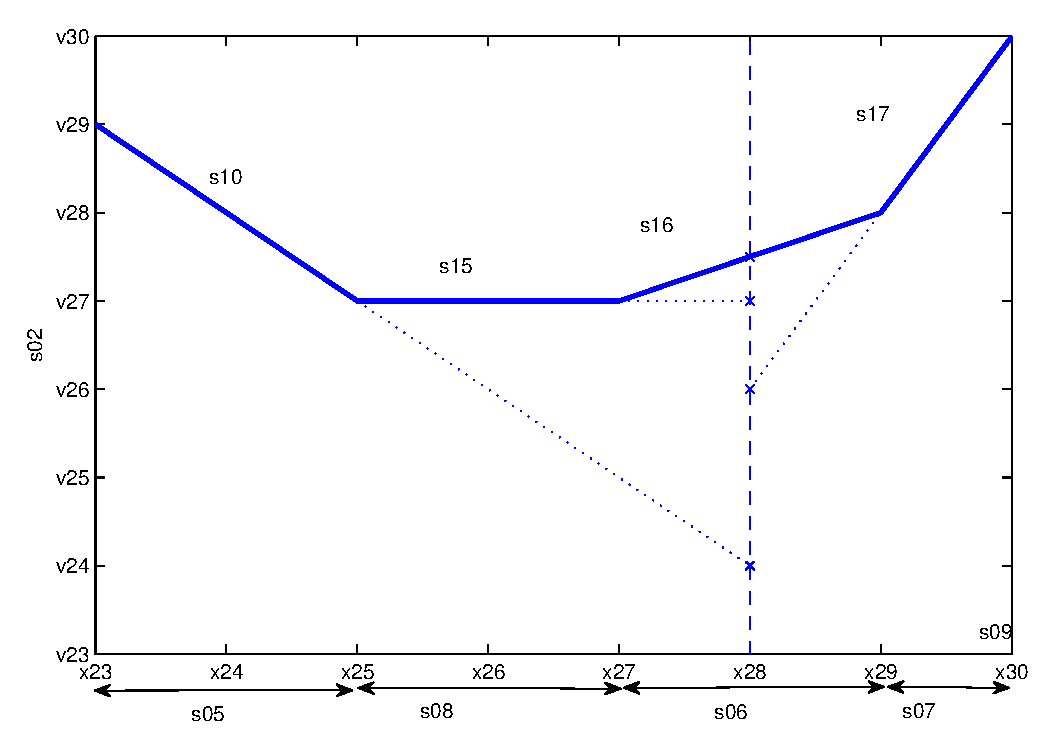
\includegraphics{onedimlp.eps}}%
\end{psfrags}%
%
% End onedimlp.tex
\end{document}
% See http://www.mathworks.de/matlabcentral/fileexchange/loadFile.do?objectId=4638
% for recent versions of laprint.m.
%
% created by:           LaPrint version 3.16 (13.9.2004)
% created on:           19-Oct-2009 10:48:43
% eps bounding box:     20 cm x 12.8261 cm
% comment:              
%
\begin{psfrags}%
\psfragscanon%
%
% text strings:
\psfrag{s02}[b][b]{\color[rgb]{0,0,0}\setlength{\tabcolsep}{0pt}\begin{tabular}{c}$J(z)$\end{tabular}}%
\psfrag{s05}[l][l]{\color[rgb]{0,0,0}\setlength{\tabcolsep}{0pt}\begin{tabular}{l}$\mathcal{R_1}$ \end{tabular}}%
\psfrag{s06}[l][l]{\color[rgb]{0,0,0}\setlength{\tabcolsep}{0pt}\begin{tabular}{l}$\mathcal{R}_3$ \end{tabular}}%
\psfrag{s07}[l][l]{\color[rgb]{0,0,0}\setlength{\tabcolsep}{0pt}\begin{tabular}{l}$\mathcal{R}_4$ \end{tabular}}%
\psfrag{s08}[l][l]{\color[rgb]{0,0,0}\setlength{\tabcolsep}{0pt}\begin{tabular}{l}$\mathcal{R}_2$ \end{tabular}}%
\psfrag{s09}[l][l]{\color[rgb]{0,0,0}\setlength{\tabcolsep}{0pt}\begin{tabular}{l}$z$ \end{tabular}}%
\psfrag{s10}[l][l]{\color[rgb]{0,0,0}\setlength{\tabcolsep}{0pt}\begin{tabular}{l}$c_1'z+d_1$ \end{tabular}}%
\psfrag{s15}[l][l]{\color[rgb]{0,0,0}\setlength{\tabcolsep}{0pt}\begin{tabular}{l}$c_2'z+d_2$ \end{tabular}}%
\psfrag{s16}[l][l]{\color[rgb]{0,0,0}\setlength{\tabcolsep}{0pt}\begin{tabular}{l}$c_3'z+d_3$ \end{tabular}}%
\psfrag{s17}[l][l]{\color[rgb]{0,0,0}\setlength{\tabcolsep}{0pt}\begin{tabular}{l}$c_4'z+d_14$ \end{tabular}}%
%
% xticklabels:
\psfrag{x01}[t][t]{0}%
\psfrag{x02}[t][t]{0.1}%
\psfrag{x03}[t][t]{0.2}%
\psfrag{x04}[t][t]{0.3}%
\psfrag{x05}[t][t]{0.4}%
\psfrag{x06}[t][t]{0.5}%
\psfrag{x07}[t][t]{0.6}%
\psfrag{x08}[t][t]{0.7}%
\psfrag{x09}[t][t]{0.8}%
\psfrag{x10}[t][t]{0.9}%
\psfrag{x11}[t][t]{1}%
\psfrag{x12}[t][t]{0}%
\psfrag{x13}[t][t]{0.1}%
\psfrag{x14}[t][t]{0.2}%
\psfrag{x15}[t][t]{0.3}%
\psfrag{x16}[t][t]{0.4}%
\psfrag{x17}[t][t]{0.5}%
\psfrag{x18}[t][t]{0.6}%
\psfrag{x19}[t][t]{0.7}%
\psfrag{x20}[t][t]{0.8}%
\psfrag{x21}[t][t]{0.9}%
\psfrag{x22}[t][t]{1}%
\psfrag{x23}[t][t]{0}%
\psfrag{x24}[t][t]{1}%
\psfrag{x25}[t][t]{2}%
\psfrag{x26}[t][t]{3}%
\psfrag{x27}[t][t]{4}%
\psfrag{x28}[t][t]{5}%
\psfrag{x29}[t][t]{6}%
\psfrag{x30}[t][t]{7}%
%
% yticklabels:
\psfrag{v01}[r][r]{0}%
\psfrag{v02}[r][r]{0.1}%
\psfrag{v03}[r][r]{0.2}%
\psfrag{v04}[r][r]{0.3}%
\psfrag{v05}[r][r]{0.4}%
\psfrag{v06}[r][r]{0.5}%
\psfrag{v07}[r][r]{0.6}%
\psfrag{v08}[r][r]{0.7}%
\psfrag{v09}[r][r]{0.8}%
\psfrag{v10}[r][r]{0.9}%
\psfrag{v11}[r][r]{1}%
\psfrag{v12}[r][r]{0}%
\psfrag{v13}[r][r]{0.1}%
\psfrag{v14}[r][r]{0.2}%
\psfrag{v15}[r][r]{0.3}%
\psfrag{v16}[r][r]{0.4}%
\psfrag{v17}[r][r]{0.5}%
\psfrag{v18}[r][r]{0.6}%
\psfrag{v19}[r][r]{0.7}%
\psfrag{v20}[r][r]{0.8}%
\psfrag{v21}[r][r]{0.9}%
\psfrag{v22}[r][r]{1}%
\psfrag{v23}[r][r]{-1}%
\psfrag{v24}[r][r]{0}%
\psfrag{v25}[r][r]{1}%
\psfrag{v26}[r][r]{2}%
\psfrag{v27}[r][r]{3}%
\psfrag{v28}[r][r]{4}%
\psfrag{v29}[r][r]{5}%
\psfrag{v30}[r][r]{6}%
%
% Figure:
\resizebox{16cm}{!}{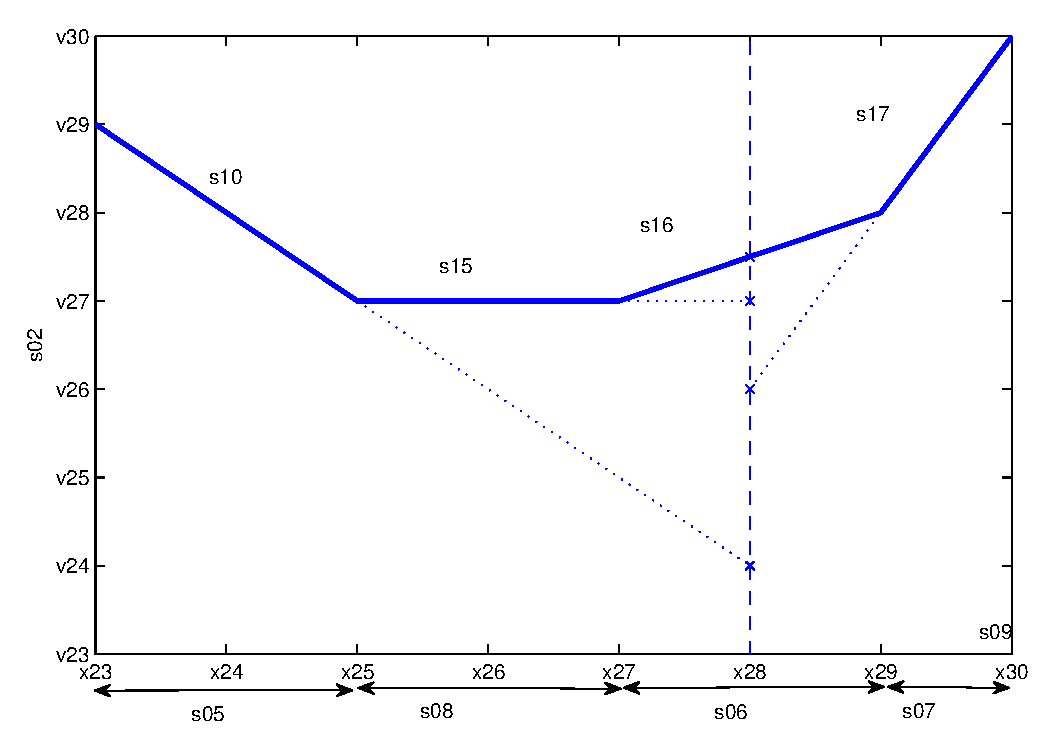
\includegraphics{onedimlp.eps}}%
\end{psfrags}%
%
% End onedimlp.tex
\end{document}
% See http://www.mathworks.de/matlabcentral/fileexchange/loadFile.do?objectId=4638
% for recent versions of laprint.m.
%
% created by:           LaPrint version 3.16 (13.9.2004)
% created on:           19-Oct-2009 10:48:43
% eps bounding box:     20 cm x 12.8261 cm
% comment:              
%
\begin{psfrags}%
\psfragscanon%
%
% text strings:
\psfrag{s02}[b][b]{\color[rgb]{0,0,0}\setlength{\tabcolsep}{0pt}\begin{tabular}{c}$J(z)$\end{tabular}}%
\psfrag{s05}[l][l]{\color[rgb]{0,0,0}\setlength{\tabcolsep}{0pt}\begin{tabular}{l}$\mathcal{R_1}$ \end{tabular}}%
\psfrag{s06}[l][l]{\color[rgb]{0,0,0}\setlength{\tabcolsep}{0pt}\begin{tabular}{l}$\mathcal{R}_3$ \end{tabular}}%
\psfrag{s07}[l][l]{\color[rgb]{0,0,0}\setlength{\tabcolsep}{0pt}\begin{tabular}{l}$\mathcal{R}_4$ \end{tabular}}%
\psfrag{s08}[l][l]{\color[rgb]{0,0,0}\setlength{\tabcolsep}{0pt}\begin{tabular}{l}$\mathcal{R}_2$ \end{tabular}}%
\psfrag{s09}[l][l]{\color[rgb]{0,0,0}\setlength{\tabcolsep}{0pt}\begin{tabular}{l}$z$ \end{tabular}}%
\psfrag{s10}[l][l]{\color[rgb]{0,0,0}\setlength{\tabcolsep}{0pt}\begin{tabular}{l}$c_1'z+d_1$ \end{tabular}}%
\psfrag{s15}[l][l]{\color[rgb]{0,0,0}\setlength{\tabcolsep}{0pt}\begin{tabular}{l}$c_2'z+d_2$ \end{tabular}}%
\psfrag{s16}[l][l]{\color[rgb]{0,0,0}\setlength{\tabcolsep}{0pt}\begin{tabular}{l}$c_3'z+d_3$ \end{tabular}}%
\psfrag{s17}[l][l]{\color[rgb]{0,0,0}\setlength{\tabcolsep}{0pt}\begin{tabular}{l}$c_4'z+d_14$ \end{tabular}}%
%
% xticklabels:
\psfrag{x01}[t][t]{0}%
\psfrag{x02}[t][t]{0.1}%
\psfrag{x03}[t][t]{0.2}%
\psfrag{x04}[t][t]{0.3}%
\psfrag{x05}[t][t]{0.4}%
\psfrag{x06}[t][t]{0.5}%
\psfrag{x07}[t][t]{0.6}%
\psfrag{x08}[t][t]{0.7}%
\psfrag{x09}[t][t]{0.8}%
\psfrag{x10}[t][t]{0.9}%
\psfrag{x11}[t][t]{1}%
\psfrag{x12}[t][t]{0}%
\psfrag{x13}[t][t]{0.1}%
\psfrag{x14}[t][t]{0.2}%
\psfrag{x15}[t][t]{0.3}%
\psfrag{x16}[t][t]{0.4}%
\psfrag{x17}[t][t]{0.5}%
\psfrag{x18}[t][t]{0.6}%
\psfrag{x19}[t][t]{0.7}%
\psfrag{x20}[t][t]{0.8}%
\psfrag{x21}[t][t]{0.9}%
\psfrag{x22}[t][t]{1}%
\psfrag{x23}[t][t]{0}%
\psfrag{x24}[t][t]{1}%
\psfrag{x25}[t][t]{2}%
\psfrag{x26}[t][t]{3}%
\psfrag{x27}[t][t]{4}%
\psfrag{x28}[t][t]{5}%
\psfrag{x29}[t][t]{6}%
\psfrag{x30}[t][t]{7}%
%
% yticklabels:
\psfrag{v01}[r][r]{0}%
\psfrag{v02}[r][r]{0.1}%
\psfrag{v03}[r][r]{0.2}%
\psfrag{v04}[r][r]{0.3}%
\psfrag{v05}[r][r]{0.4}%
\psfrag{v06}[r][r]{0.5}%
\psfrag{v07}[r][r]{0.6}%
\psfrag{v08}[r][r]{0.7}%
\psfrag{v09}[r][r]{0.8}%
\psfrag{v10}[r][r]{0.9}%
\psfrag{v11}[r][r]{1}%
\psfrag{v12}[r][r]{0}%
\psfrag{v13}[r][r]{0.1}%
\psfrag{v14}[r][r]{0.2}%
\psfrag{v15}[r][r]{0.3}%
\psfrag{v16}[r][r]{0.4}%
\psfrag{v17}[r][r]{0.5}%
\psfrag{v18}[r][r]{0.6}%
\psfrag{v19}[r][r]{0.7}%
\psfrag{v20}[r][r]{0.8}%
\psfrag{v21}[r][r]{0.9}%
\psfrag{v22}[r][r]{1}%
\psfrag{v23}[r][r]{-1}%
\psfrag{v24}[r][r]{0}%
\psfrag{v25}[r][r]{1}%
\psfrag{v26}[r][r]{2}%
\psfrag{v27}[r][r]{3}%
\psfrag{v28}[r][r]{4}%
\psfrag{v29}[r][r]{5}%
\psfrag{v30}[r][r]{6}%
%
% Figure:
\resizebox{16cm}{!}{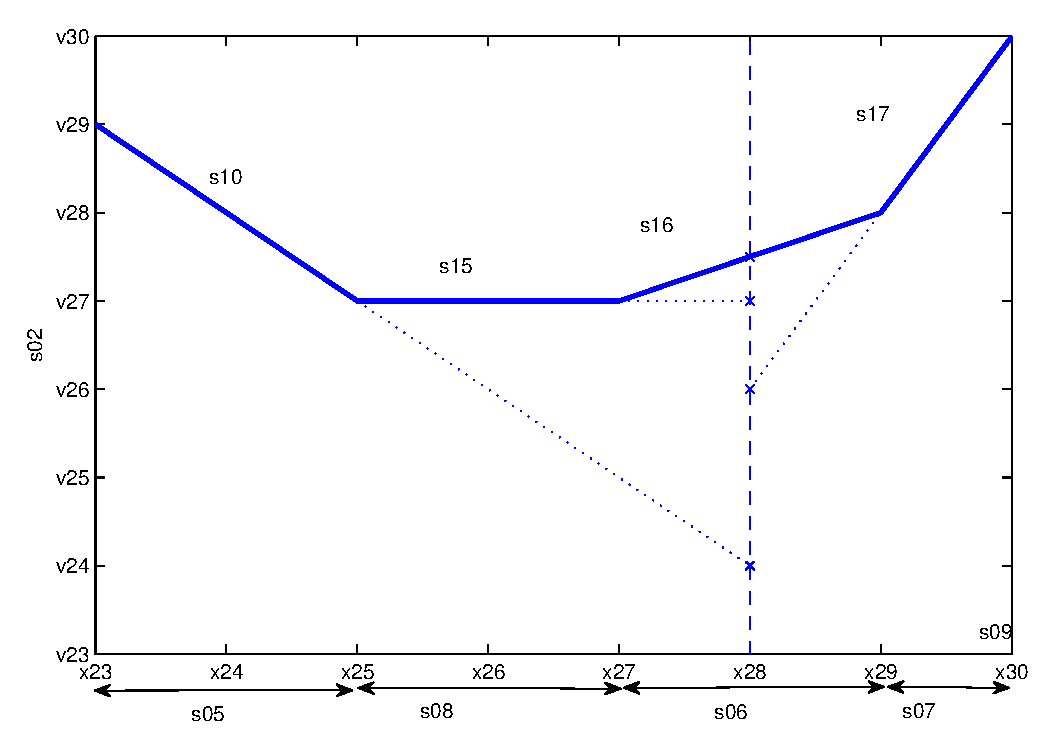
\includegraphics{onedimlp.eps}}%
\end{psfrags}%
%
% End onedimlp.tex
